% autobox-overview.tex — the two-page illustrated overview: the cycle from a message to a merge,
% and how the work is shaped. Written for someone who has not seen the box before.
%
%   pdflatex -interaction=nonstopmode autobox-overview.tex   (twice, for the TikZ positions)
%
% Plain pdflatex and psnfss fonts only — no lmodern, no templates, nothing outside texlive-latex-recommended
% and texlive-pictures. Check the result with `pdfinfo` (two pages) and `pdffonts` (all embedded).
%
% It lived in a session scratchpad for its first four versions, which meant every update began by finding
% it. Keep it here. When the box changes shape, this file is the thing to update.
\documentclass[10pt,a4paper]{article}

\usepackage[T1]{fontenc}
\usepackage[utf8]{inputenc}
\usepackage{charter}
\usepackage[scaled=0.90]{helvet}
\usepackage{courier}
\usepackage{microtype}
\usepackage[a4paper,top=1.5cm,bottom=1.3cm,left=1.8cm,right=1.8cm]{geometry}
\usepackage{xcolor}
\usepackage{tikz}
\usetikzlibrary{arrows,positioning}
\usepackage{enumitem}

\definecolor{accent}{HTML}{1F5673}
\definecolor{ink}{HTML}{22282C}
\definecolor{muted}{HTML}{5B6770}
\definecolor{line}{HTML}{9AA6AE}
\definecolor{paper}{HTML}{EDF2F5}
\definecolor{amber}{HTML}{F6E2C0}
\definecolor{amberln}{HTML}{B07C2A}
\definecolor{soft}{HTML}{F5F6F7}

\pagestyle{empty}
\setlength{\parindent}{0pt}
\setlength{\parskip}{0pt}

\newcommand{\cmd}[1]{{\small\ttfamily #1}}
\newcommand{\tcmd}[1]{{\ttfamily #1}}  % inherits the node size

% ---- shared node styles --------------------------------------------------
\tikzset{
  every node/.style={font=\sffamily},
  box/.style={draw=line,rounded corners=1.2pt,fill=white,align=center,
              font=\sffamily\scriptsize,inner sep=3pt},
  lit/.style={box,fill=paper,draw=accent},
  own/.style={box,fill=amber,draw=amberln,thick,font=\sffamily\scriptsize\bfseries},
  strip/.style={box,fill=soft,draw=line,dash pattern=on 2pt off 1.6pt},
  ar/.style={->,>=stealth,draw=accent,semithick},
  faint/.style={->,>=stealth,draw=line,semithick,dash pattern=on 2pt off 1.6pt},
  lab/.style={font=\sffamily\tiny\itshape,color=muted,inner sep=1.5pt},
  cap/.style={font=\sffamily\scriptsize\bfseries,color=accent},
}

\begin{document}

% ==========================================================================
% PAGE 1
% ==========================================================================
\begingroup\raggedright
{\sffamily\bfseries\LARGE autobox}\quad
{\sffamily\color{muted} from a Slack message to a merge, and where you come in}\\[0.35em]
{\color{line}\rule{\linewidth}{1pt}}
\endgroup

\vspace{0.4em}
{\small Claude Code is the runtime. Scripts do the bookkeeping: worktrees, commits, PRs, the board,
restarts. Models do the thinking. Every arrow below is a file on disk, not a shared context window.}

\vspace{0.6em}

\begin{center}
\begin{tikzpicture}[x=1cm,y=1.2cm]

% ---- triggers ----
\node[box,text width=4.3cm] (t1) at (2.4,0)   {\textbf{a message in \tcmd{\#repo}}\\[1pt] Slack routes it to that repo's live session};
\node[box,text width=4.3cm] (t2) at (7.8,0)   {\textbf{a timer fires}\\[1pt] pulse every 2\,h · reconcile every 20\,min · audit nightly};
\node[box,text width=4.3cm] (t3) at (13.2,0)  {\textbf{nothing is queued}\\[1pt] the session reads the standing goals};

% ---- planning session ----
\node[lit,text width=12cm] (ps) at (7.8,-1.85)
  {\textbf{PLANNING SESSION} \; one per repo, always alive in tmux \tcmd{main}\\[1.5pt]
   checks what is red, what was asked and not delivered, what the goals need. Then it sizes the work.};

\node[strip,text width=12cm] (bk) at (7.8,-0.95)
  {\tcmd{cc-broker} \; only a decision-class event wakes the session, and events that arrive together arrive as one digest, every 10--15 min};
\draw[ar] (t1.south) -- (t1.south|-bk.north);
\draw[ar] (t2.south) -- (t2.south|-bk.north);
\draw[ar] (t3.south) -- (t3.south|-bk.north);
\draw[ar] (bk.south) -- (ps.north);

% ---- sizing fan ----
\node[box,text width=4.3cm] (s1) at (2.4,-4.0)
  {\textbf{a small fix, no live track on those files}\\[1pt] the planner does it, on a short branch and a PR};
\node[box,text width=4.3cm] (s2) at (7.8,-4.0)
  {\textbf{a large read}\\[1pt] a subagent reads it and reports the conclusion; the files stay out of the planner's context};
\node[lit,text width=4.3cm] (s3) at (13.2,-4.0)
  {\textbf{open design, or a goal with several parts}\\[1pt] one worker per concern, about 5--8 files and 300--500 lines, on its own worktree and branch};

\draw[ar] (ps.south) -- (7.8,-2.95) -- (2.4,-2.95) -- (s1.north);
\draw[ar] (7.8,-2.95) -- (s2.north);
\draw[ar] (7.8,-2.95) -- (13.2,-2.95) -- (s3.north);
\node[lab] at (7.8,-2.72) {how big is it?};


% ---- worker loop ----
\node[box,text width=4.3cm] (loop) at (13.2,-6.2)
  {\textbf{\tcmd{cc-loop}}, headless\\[1pt] a fresh \tcmd{claude -p} each iteration, briefed from \tcmd{task.md} and the tail of \tcmd{progress.md} · capped by budget and turns · ends in a PR or a BLOCKED question};
\draw[ar] (s3.south) -- (loop.north);

\node[box,text width=3.4cm] (pr) at (7.8,-7.6) {\textbf{PULL REQUEST}};
\draw[ar] (loop.west) -- (10.6,-6.2) -- (10.6,-7.6) -- (pr.east);
\draw[ar] (s1.south) -- (2.4,-7.6) -- (pr.west);

% ---- landing pipeline ----
\node[box,text width=10.5cm] (g) at (7.8,-9.0)
  {\textbf{GATES} \; the full suite, against the PR's own head in a throwaway worktree. Several PRs gate and review at once; only merge, install and restart are serial.};
\node[box,text width=10.5cm] (rv) at (7.8,-10.3)
  {\textbf{REVIEW} \; a second model reads the diff against the brief's done-criteria, once per change rather than once per push. It does not read the worker's journal.};
\node[own,text width=10.5cm] (ow) at (7.8,-11.65)
  {YOU \; one reaction in \tcmd{\#approvals}};
\node[lit,text width=10.5cm] (ld) at (7.8,-13.0)
  {\textbf{\tcmd{cc-land}}, the only thing that merges \; squash · \tcmd{install.sh} · restart the units the change added · check the ask was delivered};

\draw[ar] (pr.south) -- (g.north);
\draw[ar] (g.south) -- (rv.north);
\draw[ar] (rv.south) -- (ow.north);
\draw[ar] (ow.south) -- (ld.north);

% ---- guard bracket ----
\draw[draw=line,semithick] (0.35,-5.3) -- (0.05,-5.3) -- (0.05,-13.6) -- (0.35,-13.6);
\node[rotate=90,font=\sffamily\tiny,color=muted,anchor=south] at (0.05,-9.45)
  {\tcmd{cc-guard}, a hook: blocks merge, deploy, sudo, force-push, edits outside the worktree};

% ---- return rail ----
\draw[ar] (ld.east) -- (16.4,-13.0) -- (16.4,0.55) -- (13.2,0.55) -- (t3.north);
\node[rotate=90,lab,anchor=south] at (16.4,-6.3)
  {\tcmd{cc-reconcile}, every 20 min: compares the board with the box and writes one snapshot};

% ---- durable state strip ----
\node[strip,text width=15.1cm] (st) at (7.8,-14.6)
  {\textbf{THE FILES THAT CARRY STATE}\\[2pt]
   \tcmd{task.md} the brief \, · \, \tcmd{progress.md} the journal \, · \, the board (JSON, per repo) \, · \, git and the PR \, · \, \tcmd{reconcile.json}, the one snapshot that \tcmd{cc~ls}, the digest and the Slack Home tab all render};
\draw[faint] (7.8,-13.62) -- (7.8,-14.02);
\draw[faint] (loop.south) -- (13.2,-7.05) -- (15.7,-7.05) -- (15.7,-14.6) -- (st.east);

\end{tikzpicture}
\end{center}

\vspace{0.3em}

{\small
A worker and its reviewer never share a context window. They share files, so any session can be
killed and restarted and the work is still there. You appear once, at the reaction, and only for the
cases listed on the back. The rest runs from timers and hooks.}

\newpage

% ==========================================================================
% PAGE 2
% ==========================================================================
\begingroup\raggedright
{\sffamily\bfseries\Large How the work is shaped}\\[0.3em]
{\color{line}\rule{\linewidth}{1pt}}
\endgroup

\vspace{0.8em}
{\sffamily\bfseries\color{accent} 1 \; The glue shrinks as Claude Code grows}

\vspace{0.45em}
\begin{center}
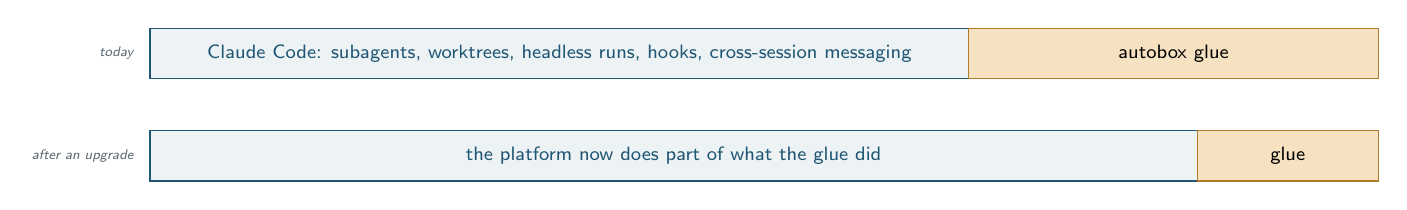
\begin{tikzpicture}[x=1cm,y=1cm]
\node[lab,anchor=east] at (-0.15,0) {today};
\draw[fill=paper,draw=accent] (0,-0.32) rectangle (10.4,0.32);
\node[font=\sffamily\scriptsize,color=accent] at (5.2,0) {Claude Code: subagents, worktrees, headless runs, hooks, cross-session messaging};
\draw[fill=amber,draw=amberln] (10.4,-0.32) rectangle (15.6,0.32);
\node[font=\sffamily\scriptsize] at (13.0,0) {autobox glue};

\node[lab,anchor=east] at (-0.15,-1.3) {after an upgrade};
\draw[fill=paper,draw=accent] (0,-1.62) rectangle (13.3,-0.98);
\node[font=\sffamily\scriptsize,color=accent] at (6.65,-1.3) {the platform now does part of what the glue did};
\draw[fill=amber,draw=amberln] (13.3,-1.62) rectangle (15.6,-0.98);
\node[font=\sffamily\scriptsize] at (14.45,-1.3) {glue};
\end{tikzpicture}
\end{center}

\vspace{0.15em}
{\small On each model upgrade, try deleting one workaround. Each one encodes an assumption about a
model weakness, and those expire. Nothing is built that the platform already ships. The board
overlaps native agent teams and goes when that feature is GA.}

\vspace{0.9em}
{\sffamily\bfseries\color{accent} 2 \; Sizing the work}

\vspace{0.45em}
\begin{center}
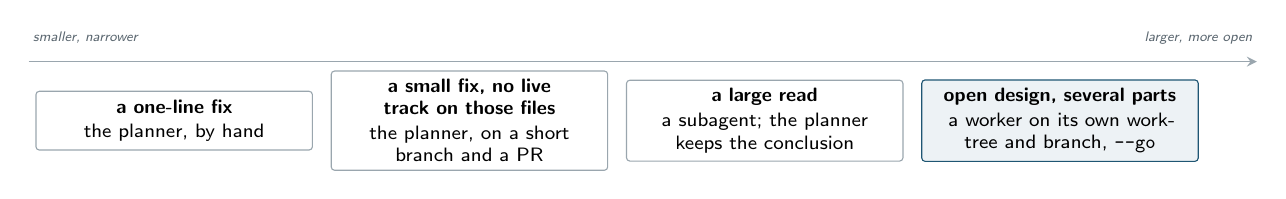
\begin{tikzpicture}[x=1cm,y=1cm]
\draw[->,>=stealth,draw=line,semithick] (0,0.75) -- (15.6,0.75);
\node[lab,anchor=west] at (0,1.05) {smaller, narrower};
\node[lab,anchor=east] at (15.6,1.05) {larger, more open};

\node[box,text width=3.3cm] at (1.85,0) {\textbf{a one-line fix}\\[1pt] the planner, by hand};
\node[box,text width=3.3cm] at (5.6,0) {\textbf{a small fix, no live track on those files}\\[1pt] the planner, on a short branch and a PR};
\node[box,text width=3.3cm] at (9.35,0) {\textbf{a large read}\\[1pt] a subagent; the planner keeps the conclusion};
\node[lit,text width=3.3cm] at (13.1,0) {\textbf{open design, several parts}\\[1pt] a worker on its own worktree and branch, \tcmd{-{}-go}};
\end{tikzpicture}
\end{center}

\vspace{0.25em}
{\small Two workers never edit the same file at the same time. That has happened twice. Each time it
cost a rebase, and the same fix was written twice. Split by file, or run those in sequence. Otherwise
prefer fewer, larger runs: one concern per worker, about 5 to 8 files and 300 to 500 lines, each on
its own worktree and branch. A brief says what, why, the boundaries, and how done will be judged. The
worker decides the steps. The reviewer checks the diff against those done-criteria. A brief that
prescribes the steps instead is refused at the dispatch door by a small model that reads it first ---
the rule was written down twice and followed neither time, so it stopped being a rule and became a gate.}

\vspace{0.9em}
{\sffamily\bfseries\color{accent} 3 \; Handoffs}

\vspace{0.45em}
\begin{center}
\begin{tikzpicture}[x=1cm,y=1cm]
% lane labels
\node[lab,anchor=east,text width=1.8cm,align=right] at (1.95,0)     {a session with a live window};
\node[lab,anchor=east,text width=1.8cm,align=right] at (1.95,-1.45) {its successor};
\node[lab,anchor=east,text width=1.8cm,align=right] at (1.95,-2.75) {a headless worker};

% predecessor lane
\node[box,text width=3.2cm] (p1) at (3.75,0)
  {\tcmd{cc-context} reads the context used off the transcript after every turn\\[1pt] 30\% journal · 40\% hand off · 60\% hand off regardless};
\node[box,text width=2.75cm] (p2) at (7.0,0)
  {past 40\%: finishes what is in flight, then a successor is started};
\node[box,text width=3.2cm] (p3) at (10.35,0)
  {keeps working and still owns the channel; answers what the successor asks};
\node[box,text width=3.2cm] (p4) at (13.85,0)
  {renamed \tcmd{\textasciitilde old}; drains for 10 min, anything typed into it is relayed; then its window ends};
\draw[ar] (p1) -- (p2);
\draw[ar] (p2) -- (p3);
\draw[ar] (p3) -- (p4);

% successor lane
\node[lit,text width=3.2cm] (s1) at (10.35,-1.45)
  {starts alongside on one packet from \tcmd{cc-handoff -{}-brief}, then asks the predecessor only what no file holds};
\node[lit,text width=3.2cm] (s2) at (13.85,-1.45)
  {runs \tcmd{cc-handoff -{}-ready}: one atomic swap of the record file; it now owns the channel};
\draw[ar] (s1) -- (s2);
\draw[<->,>=stealth,draw=line,semithick,dash pattern=on 2pt off 1.6pt] (p3.south) -- (s1.north);
\draw[ar] (p2.south) -- (7.0,-1.45) -- (s1.west);

% cutover
\draw[draw=accent,semithick,dash pattern=on 2pt off 1.6pt] (12.1,0.85) -- (12.1,-2.15);
\node[lab,color=accent,anchor=south] at (12.1,0.85) {cutover};
\node[lab,anchor=south] at (10.35,0.72) {overlap: both alive};

% headless worker lane
\node[strip,text width=13.3cm] (w) at (8.8,-2.75)
  {\textbf{never handed off.} Each \tcmd{cc-loop} iteration is a fresh \tcmd{claude -p} that reads the same \tcmd{progress.md}. Past a line it is only told to journal.};
\end{tikzpicture}
\end{center}

\vspace{0.25em}
{\small A takeover costs a few turns rather than seventy: the brief packet is the last journal entry,
the unfinished board, what is landing, the live workers, the open PRs and the open asks, in one read.
Crossing 40\% restarts nothing by itself. The successor starts at the first turn with nothing
in flight, because nothing records half-done work. Ownership moves only on a successful
\cmd{cc-handoff -{}-ready}, so any failure leaves the predecessor in charge. A worker's loop and a
session's handoff read the same journal.}

\vspace{0.9em}
{\sffamily\bfseries\color{accent} 4 \; Other people on the box}

\vspace{0.45em}
\begin{center}
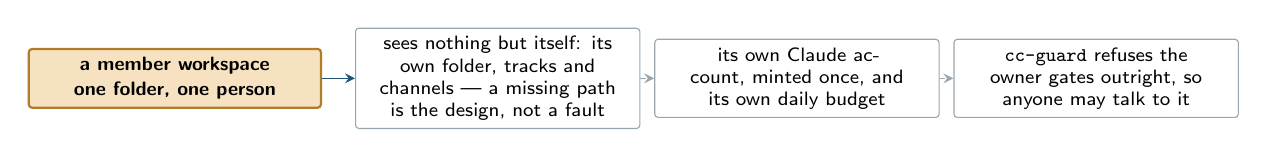
\begin{tikzpicture}[x=1cm,y=1cm]
\node[own,text width=3.5cm] (mw) at (2.0,0) {a member workspace\\[1pt] one folder, one person};
\node[box,text width=3.4cm] (m1) at (6.1,0) {sees nothing but itself: its own folder, tracks and channels --- a missing path is the design, not a fault};
\node[box,text width=3.4cm] (m2) at (9.9,0) {its own Claude account, minted once, and its own daily budget};
\node[box,text width=3.4cm] (m3) at (13.7,0) {\tcmd{cc-guard} refuses the owner gates outright, so anyone may talk to it};
\draw[ar] (mw) -- (m1);
\draw[faint] (m1) -- (m2);
\draw[faint] (m2) -- (m3);
\end{tikzpicture}
\end{center}

\vspace{0.25em}
{\small Each workspace runs in its own sandbox, so a session inside one cannot read the rest of the box
and never asks you for what the sandbox already contains. It reaches you the same way anything else
does. Five exist today.}

\vspace{0.9em}
{\sffamily\bfseries\color{accent} 5 \; Where you are still needed}

\vspace{0.4em}
\begin{center}
\begin{tikzpicture}[x=1cm,y=1cm]
\node[own,text width=15.0cm,font=\sffamily\scriptsize] at (7.8,0)
 {\textbf{Deploying \; · \; spend over budget \; · \; host, network or service changes \; · \; anything destructive}\\[2.5pt]
  \textbf{anything sent outward in your name \; · \; anything that widens what a non-owner may do}\\[2.5pt]
  \textbf{anything that opens the box to the outside: an SSH path, a port, a tunnel, a new connector}};
\end{tikzpicture}
\end{center}

\vspace{0.3em}
{\small That list is all of it. Everything else the box decides on its own. When it needs you it
@-mentions you in Slack, which reaches your phone. A line in a terminal or a row on a board does not.
\cmd{cc-guard} enforces the list as a hook, so no prompt can talk a session past it.}

\vfill
{\scriptsize\color{muted} Longer version: \cmd{autobox.pdf}. Sources: \cmd{core/docs/DESIGN.md},
\cmd{core/docs/WORKING.md}, \cmd{core/README.md}.}

\end{document}
